\documentclass[lettersize,journal]{IEEEtran}
\usepackage{hyperref}
\usepackage{amsmath,amsfonts}
\usepackage{algorithmic}
\usepackage{algorithm}
\usepackage{array}
\usepackage[caption=false,font=normalsize,labelfont=sf,textfont=sf]{subfig}
\usepackage{textcomp}
\usepackage{stfloats}
\usepackage{url}
\usepackage{verbatim}
\usepackage{graphicx}
\usepackage[font=footnotesize,justification=centering]{caption}
\usepackage{cite}
\hyphenation{op-tical net-works semi-conduc-tor IEEE-Xplore}
% updated with editorial comments 8/9/2021
\usepackage{subfig}
\usepackage{amssymb}





\begin{document}





\title{Post Delivery Robot Simulation using Monte Carlo}

\author{Mohamad Ali Saber \\ \href{mailto:malisaber@yahoo.com}{malisaber@yahoo.com}}
\maketitle

\begin{abstract}
In this computer assignment, we dive into find the optimal policy for a Post Delivery Robot using Monte Carlo (MC) algorithm. The RL agent is a car in a 5 by 5 grid world environment trying to pick up the postal package in one of the pre-defined location. The agent interacts with the environment to find the best action in each state. It can move in the four main direction that are North, East, South, and West and also pick up a package. It receives a reward based on the action that it takes. The reward function generates in a way that guide the agent to find the shortest path to the postal box and punished it whenever it picks the wrong box.\par

The objective of this computer assignment is to develop and compare On-Policy and Off-Policy MC control algorithm for policy improvement. Both algorithms deploy the First-Visit MC updates find the best strategy on 100,000 different episodes. The on-policy uses an $\epsilon-greedy$ while the off-policy uses an $\epsilon-greedy$ policy to learn and update the deterministic target policy.\par

To visualize the results, the action map and state value of each different location of the postal package for two learning methods have been plotted. And lastly, to have a comparison between these two methods, the average return of each algorithm per episode have been plotted. The results show that the off-policy could find the optimum policy while the on-policy failed to find even the near optimum policy. But, using some technique to fine-tuning the on-policy helps to find the optimum policy using this method either.
\end{abstract}

\begin{IEEEkeywords}
Reinforcement Learning, Monte Carlo, First-visit, Policy.
\end{IEEEkeywords}




%%%%%%%%%%%%%%%%%%%%%%%%%%%%%%%%%%%%%%%%%%%%%%%%%%%%%%%%%%%%%%%%%%%%%%%%%%%%%%%%%%
%                   INTERODUCTION
%%%%%%%%%%%%%%%%%%%%%%%%%%%%%%%%%%%%%%%%%%%%%%%%%%%%%%%%%%%%%%%%%%%%%%%%%%%%%%%%%%
\section{Introduction}
\IEEEPARstart{K}{nowledge} of environment helps the humankind to propose a complete model of that environment and also have a perfect and complete control over that environment, but in some cases, the under study environment become too complex to find the mathematical model of that environment or calculating the mathematical model of it becomes too computationally intensive that proposing the model is not a cost-efficient task. Basic Reinforcement Learning algorithms use the complete model of environment to find the best control over that, but those algorithms fail when there is no accurate or complete model available. in this case, scientists propose a new types of RL algorithms that learns from the previous experience of an agent within that environment to find the best action in each states of the environment. Monte carlo On-Policy and Off-Policy are model-free and experiment-based learning algorithms that learns the near best and best action from directly interacting with the environment, respectively.\par

The environment is a 5×5 discrete grid representing the operational area of a delivery robot. The robot can move north, south, east, or west, or attempt to pick up a package using a fifth action. Any attempts to exit the world is useless and brings the robot to its last location. At the start of each episode, the robot's position is randomized, and the package is placed at one of four fixed places. The robot's actions are deterministic, but any attempt to move outside the grid results in a penalty. Also, there are some walls within the grid world that limits the movement of the robot, by punishing the robot every times that it hits any of these walls, the robot learns to move around them when any wall is in its path.\par

The episode ends either when the package is picked up successfully or after 25 steps. The reward structure encourages efficient and accurate behavior, with +20 for a correct pickup, –10 for illegal moves (i.e. exiting the world and hitting the walls) or incorrect pickups, and –1 for each time step to discourage delays. This environment provides a clear, structured setting for training and evaluating Monte Carlo control algorithms. \par




The following of this report is organized az:
\begin{itemize}
    \item Section II: methodology of the solution
    \item Section III: a brief explanation of the implemented code
    \item Section IV: simulation results
    \item Section V: Conclusion
\end{itemize}
\vspace{0.3cm}


%%%%%%%%%%%%%%%%%%%%%%%%%%%%%%%%%%%%%%%%%%%%%%%%%%%%%%%%%%%%%%%%%%%%%%%%%%%%%%%%%%
%                  Methodology
%%%%%%%%%%%%%%%%%%%%%%%%%%%%%%%%%%%%%%%%%%%%%%%%%%%%%%%%%%%%%%%%%%%%%%%%%%%%%%%%%%
\section{Methodology}
In this section, a brief explanation of the model will be presented. This section contains four subsections to cover the state model, action model, reward model, and Environment model of the RL agent.\par

\subsection{State Model}
The state model should covers all the possible configurations of the car and the postal package position. Since the world is a 5 by 5 discrete environment it can have 25 distinguishable positions and therefore 25 different positions to represent the coordinates of the robot. Also there is 4 different possible locations for the package that has a direct effect on the agent behavior and should be concluded as the state of the environment. Therefore, the state vector defined as below with total 100 possible different states.

\begin{equation}
S = [x, y, p]
\end{equation}

where x and y denote as the x and y coordinate of the car, respectively, and p represents the number of package. 

\subsection{Action Model}
To have the full access to each position of the map, the robot should be capable of moving in all 4 main directions as North, East, South, and West. The fifth action defined as picking up the package. Therefore, the action space defined as bellow:

\begin{equation}
A = [N, E, S, W, P]
\end{equation}


\subsection{Reward Model}
The agent required to find the shortest path to the package, avoid hitting to the wall, staying within the world, and pick up the right package. To guide the agent to achieve these goals, the reward function describes as following, a -1 reward to each action within the world, -10 points when the agent tries to leave the world, hitting the inner walls, and picking the wrong package, and last, a +20 when it picks the right package. 


\subsection{Environment Model}
Environment modeled through its 4-argument transition probability function. Therefore environment uses its transition probability to find the next state and reward based on present state and taken action.  


%%%%%%%%%%%%%%%%%%%%%%%%%%%%%%%%%%%%%%%%%%%%%%%%%%%%%%%%%%%%%%%%%%%%%%%%%%%%%%%%%%
%                 Implementation
%%%%%%%%%%%%%%%%%%%%%%%%%%%%%%%%%%%%%%%%%%%%%%%%%%%%%%%%%%%%%%%%%%%%%%%%%%%%%%%%%%
\section{Implementation}
In this section, three main implemented functions that are Environment class, On-Policy and Off-Policy, will be explained.



\subsection{Environment}
The Environment class has been developed, this class contains some physical information of the environment like position of the robot and package and dynamics of the environment, and other intellectual information like episode length etc. This class contains some fundamental function to generate and simulate the environment using the given policy, and also plot the results. Figure \ref{fig:env_class} shows some implemented function within the environment class and figure \ref{fig:env} shows a frame of simulation.


\begin{figure}
    \centering
    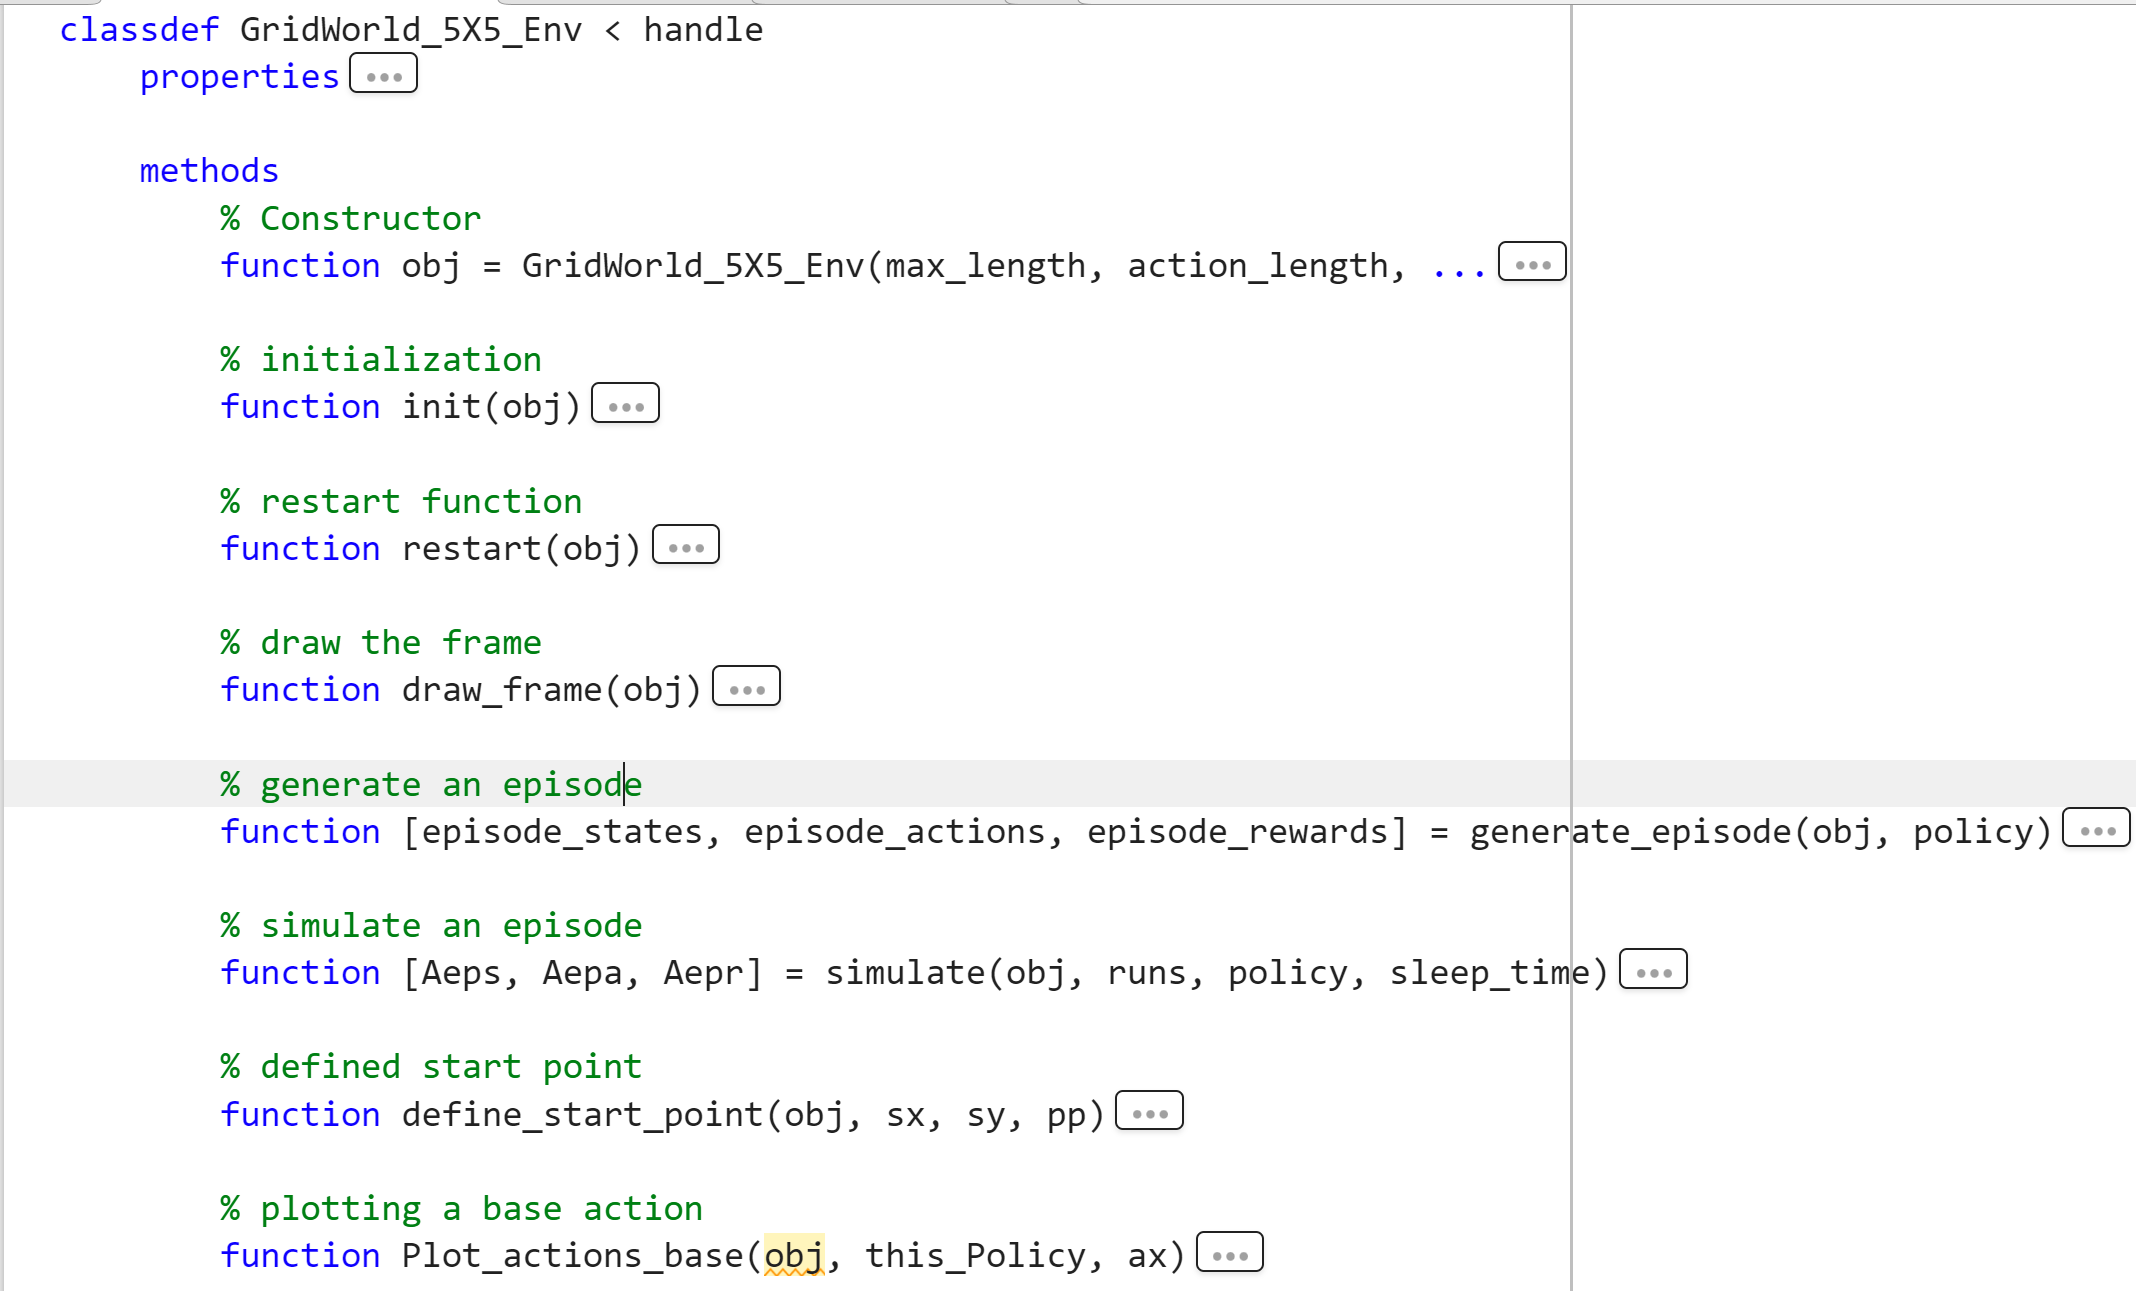
\includegraphics[width=0.9\linewidth]{pics/env_class.PNG}
    \caption{\centering some function of the environment class}
    \label{fig:env_class}
\end{figure}

\begin{figure}
    \centering
    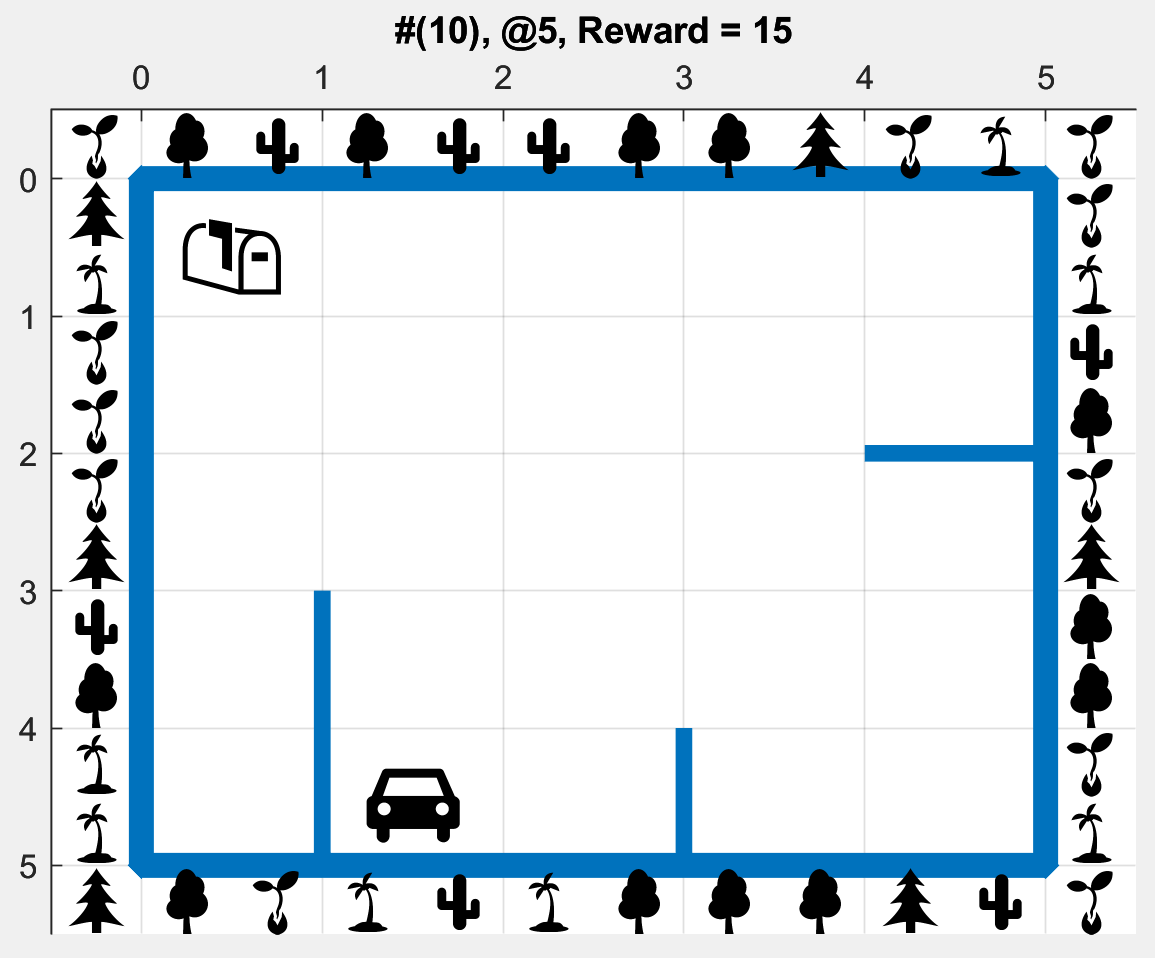
\includegraphics[width=0.9\linewidth]{pics/env.PNG}
    \caption{\centering a simulation frame}
    \label{fig:env}
\end{figure}



\subsection{On-Policy}
The on-policy algorithm implemented under a function with the same name. Within the function, at each episode, the environment resets and the package and the robot respawn randomly. Then the environment generate a trajectory using the given policy and for each step of that trajectory, action-value of corresponded episode updates. This routine repeats for 100,000 times and then returns the generated policy and corresponded action-value matrix. 



\subsection{Off-Policy}
Off-policy algorithm declared in separate file, the overall structure of off-policy function is the same as the on-policy function with minor difference in the updating of action-value matrix. 


In the main script, at first, some variables have been initialized, then the dynamics of the environment has been generated and after that, an instantiation of the environment has been instanced. and at the end, two different policies using on-policy and off-policy generates and the environment simulated 10 times using those policies.


%%%%%%%%%%%%%%%%%%%%%%%%%%%%%%%%%%%%%%%%%%%%%%%%%%%%%%%%%%%%%%%%%%%%%%%%%%%%%%%%%%
%                  simulation results
%%%%%%%%%%%%%%%%%%%%%%%%%%%%%%%%%%%%%%%%%%%%%%%%%%%%%%%%%%%%%%%%%%%%%%%%%%%%%%%%%%
\section{simulation results}
Both MC control algorithm learn on 100,000 episodes, with $\gamma$ of 1. The $\epsilon$ in the on-policy was 0.01 while in the off-policy was 0.3 . The predicted policy using on-policy MC control method depicted in figure \ref{fig:onp_act} and as you can see, it contains some irregular behaviors like switching between two adjacent states like selected state in top-right part. The state value color map of this method shows in figure \ref{fig:onp_sv}. The policy that off-policy MC control method generated is optimum and does not contains and un-optimum or unusual behaviors. The action map and state value color map of this method depicted in figure \ref{fig:ofp_act} and \ref{fig:ofp_sv}, respectively.


\begin{figure}
    \centering
    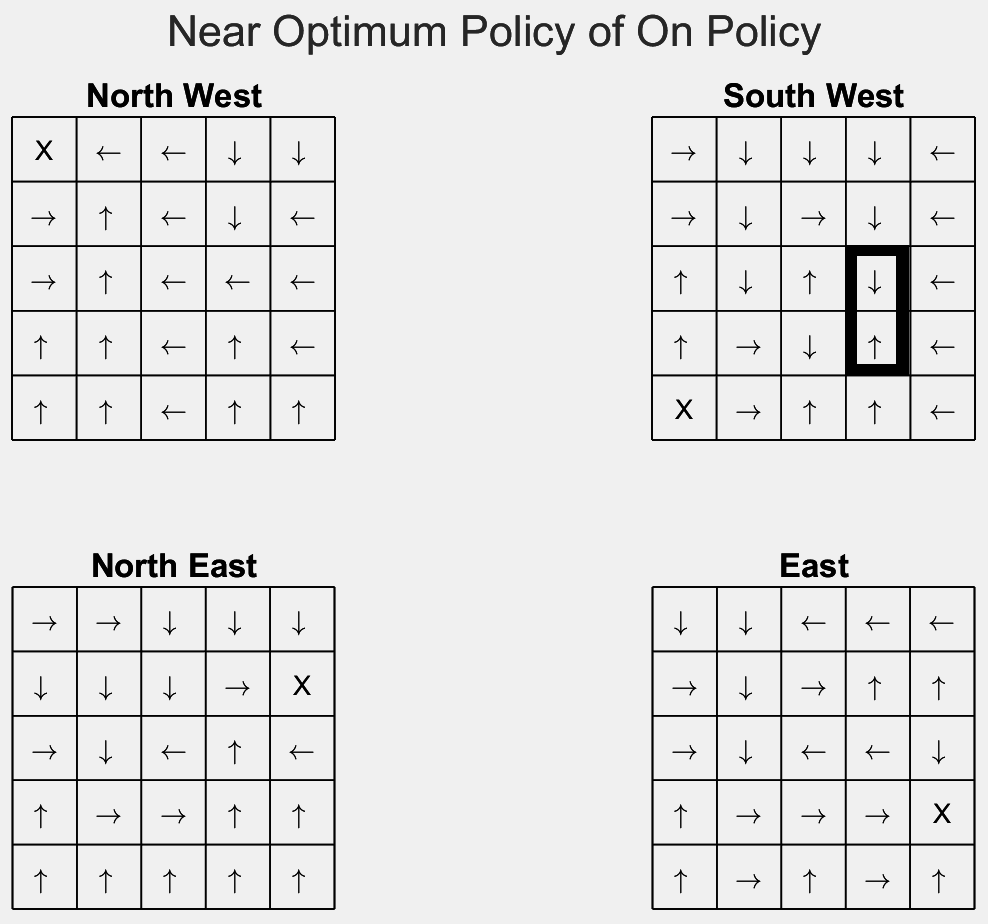
\includegraphics[width=0.9\linewidth]{pics/onp_act.PNG}
    \caption{\centering Action Map of on-policy predicted policy for different package positions}
    \label{fig:onp_act}
\end{figure}

\begin{figure}
    \centering
    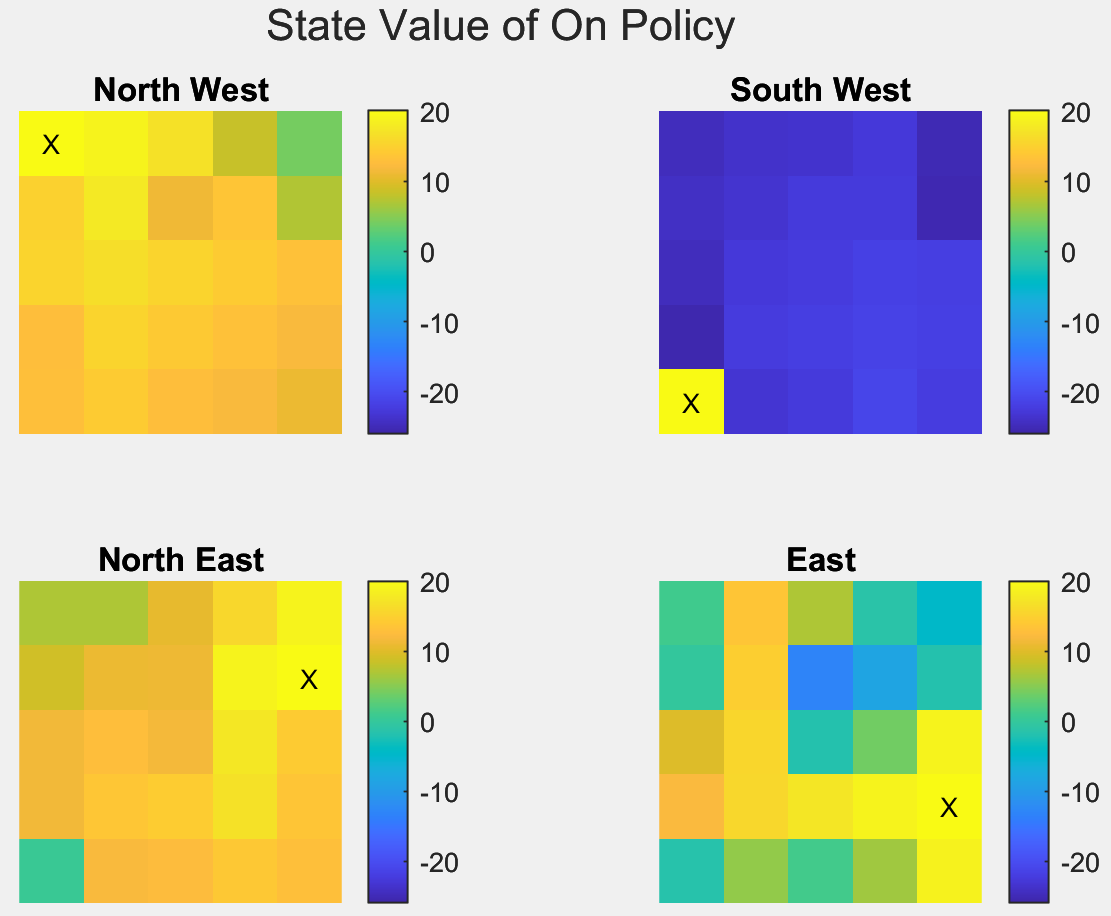
\includegraphics[width=0.9\linewidth]{pics/onp_state_val.PNG}
    \caption{\centering Color map of on-policy estimated state value for different package positions}
    \label{fig:onp_sv}
\end{figure}


\begin{figure}
    \centering
    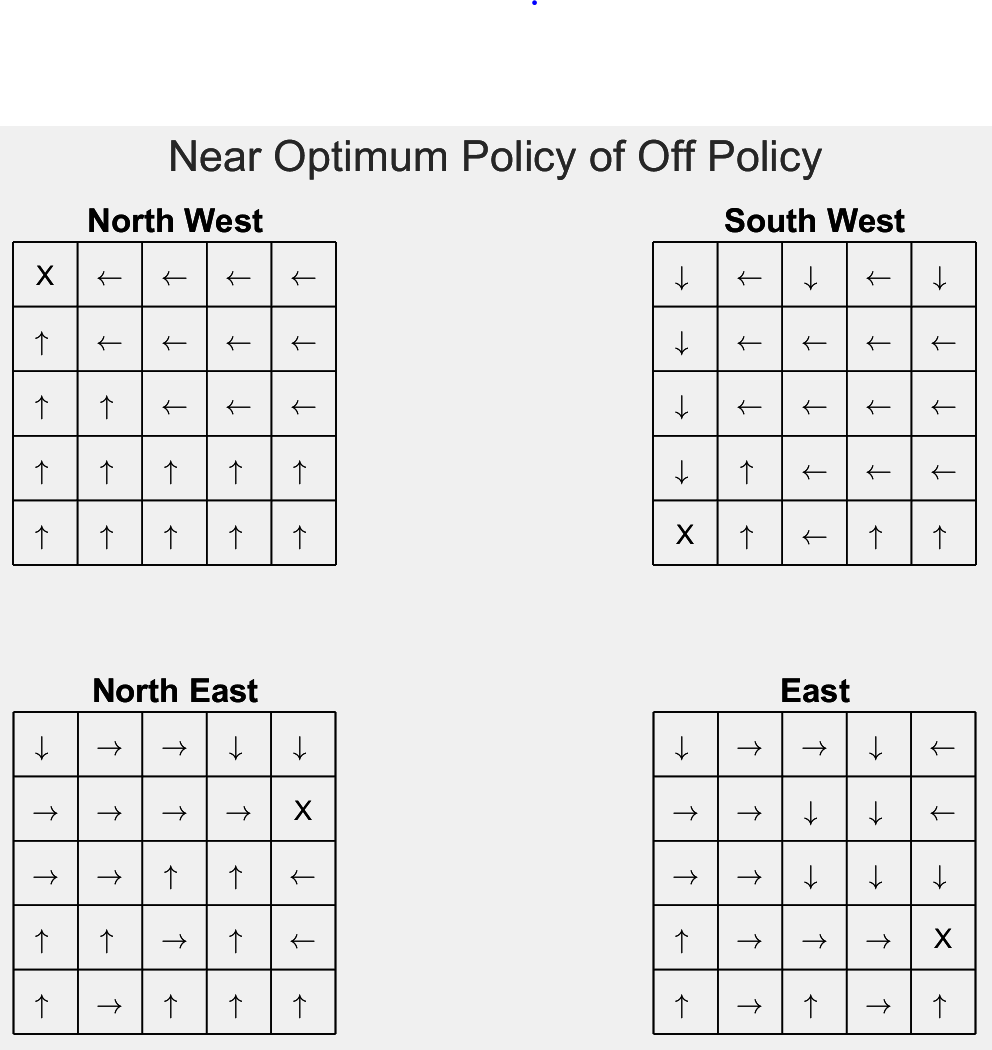
\includegraphics[width=0.9\linewidth]{pics/ofp_act.PNG}
    \caption{\centering Action Map of off-policy predicted policy for different package positions}
    \label{fig:ofp_act}
\end{figure}

\begin{figure}
    \centering
    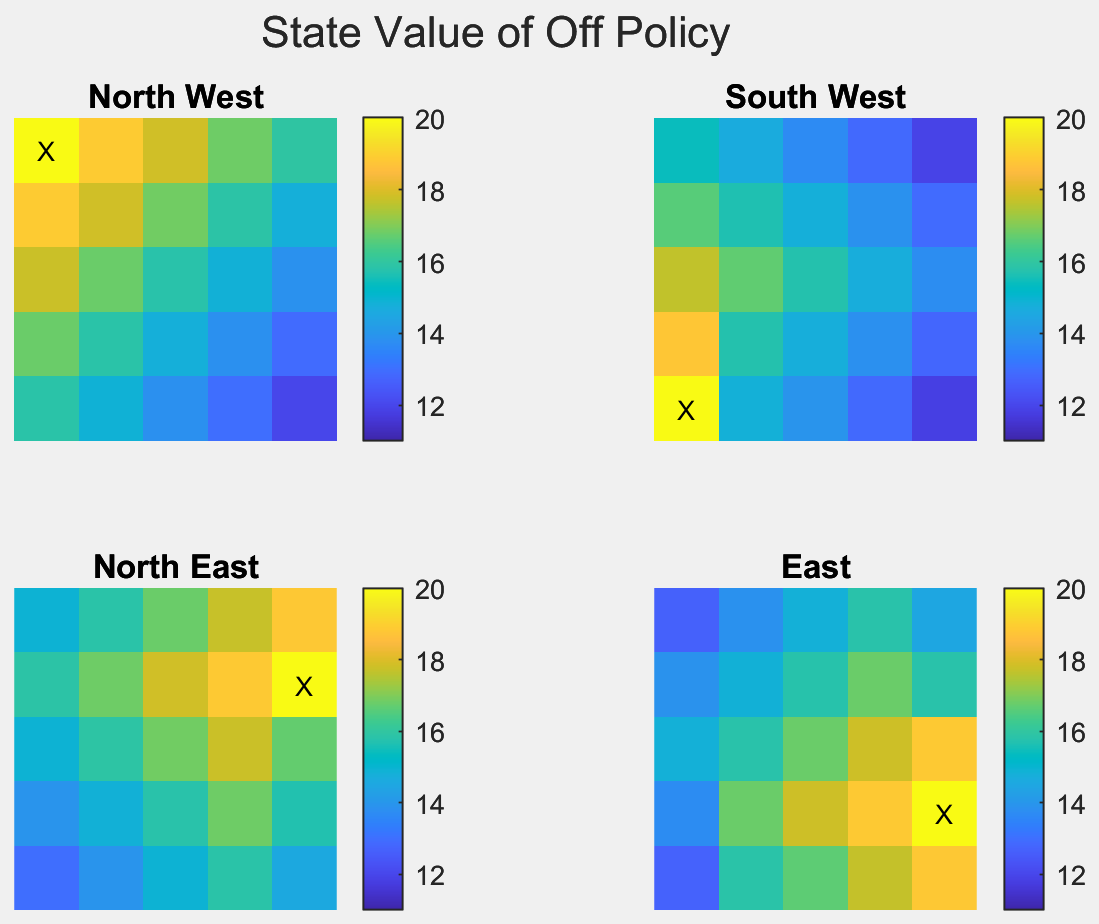
\includegraphics[width=0.9\linewidth]{pics/ofp_state_val.PNG}
    \caption{\centering Color map of off-policy estimated state value for different package positions}
    \label{fig:ofp_sv}
\end{figure}


One of the challenges encountered in the on-policy Monte Carlo (MC) control method was its inability to reliably discover the optimal policy. This issue arose when the agent selected suboptimal actions during training, causing the step size for updating the average return of those actions to become very small. As a result, even if the optimal action was occasionally chosen at random, the positive reward it yielded had minimal influence on the estimated action value. Consequently, the on-policy method often failed to converge to the best action in each state.\par

To overcome this limitation, the learning process was divided into several smaller training phases. In each phase, the policy learned from the previous phase was used as the starting point and further refined using the same on-policy MC algorithm. Simulation results showed that this staged approach enabled the on-policy method to converge to the optimal action in each state, achieving performance comparable to the off-policy method—even without decaying $\epsilon$ over time. Specifically, the training was split into 10 segments of 10,000 episodes each, with $\epsilon$ set to 1/(10 * process number). The resulting action maps and state-value heatmaps for this method are shown in Figures \ref{fig:Aonp_act} and \ref{fig:Aonp_sv}, respectively.\par


\begin{figure}
    \centering
    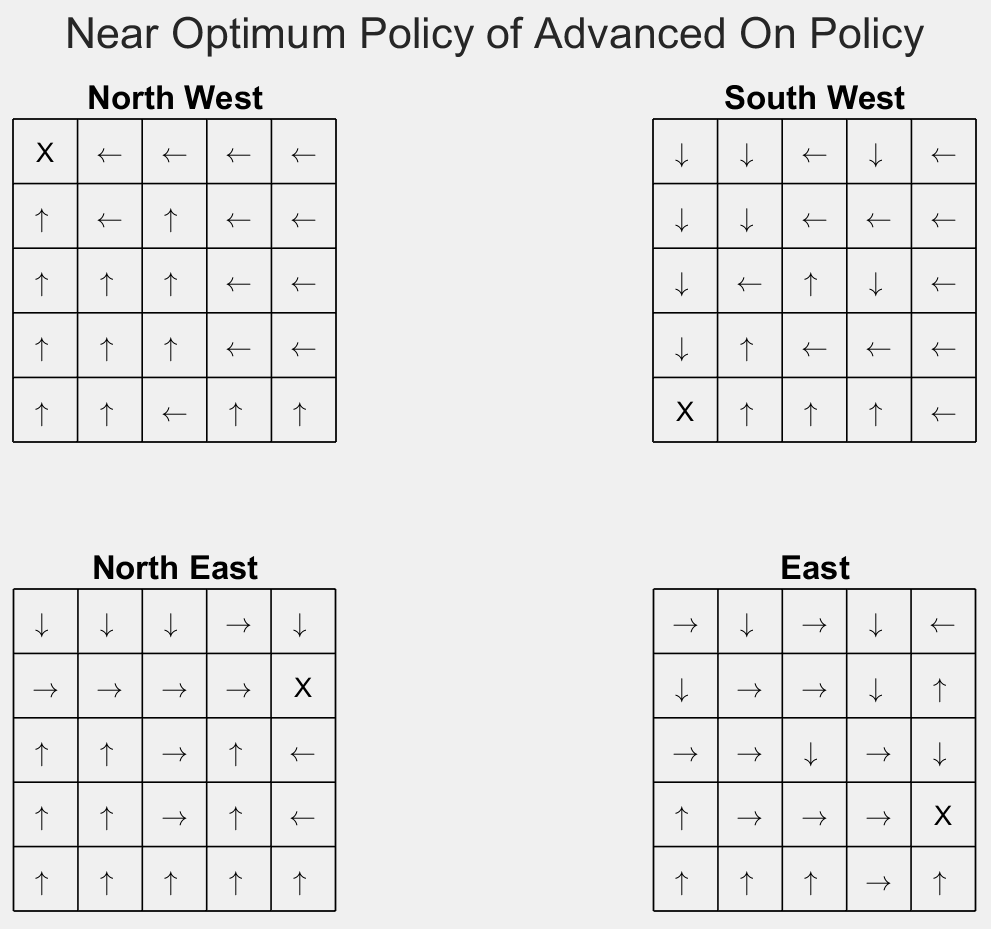
\includegraphics[width=0.9\linewidth]{pics/Aonp_act.PNG}
    \caption{\centering Action Map of advanced on-policy predicted policy for different package positions}
    \label{fig:Aonp_act}
\end{figure}

\begin{figure}
    \centering
    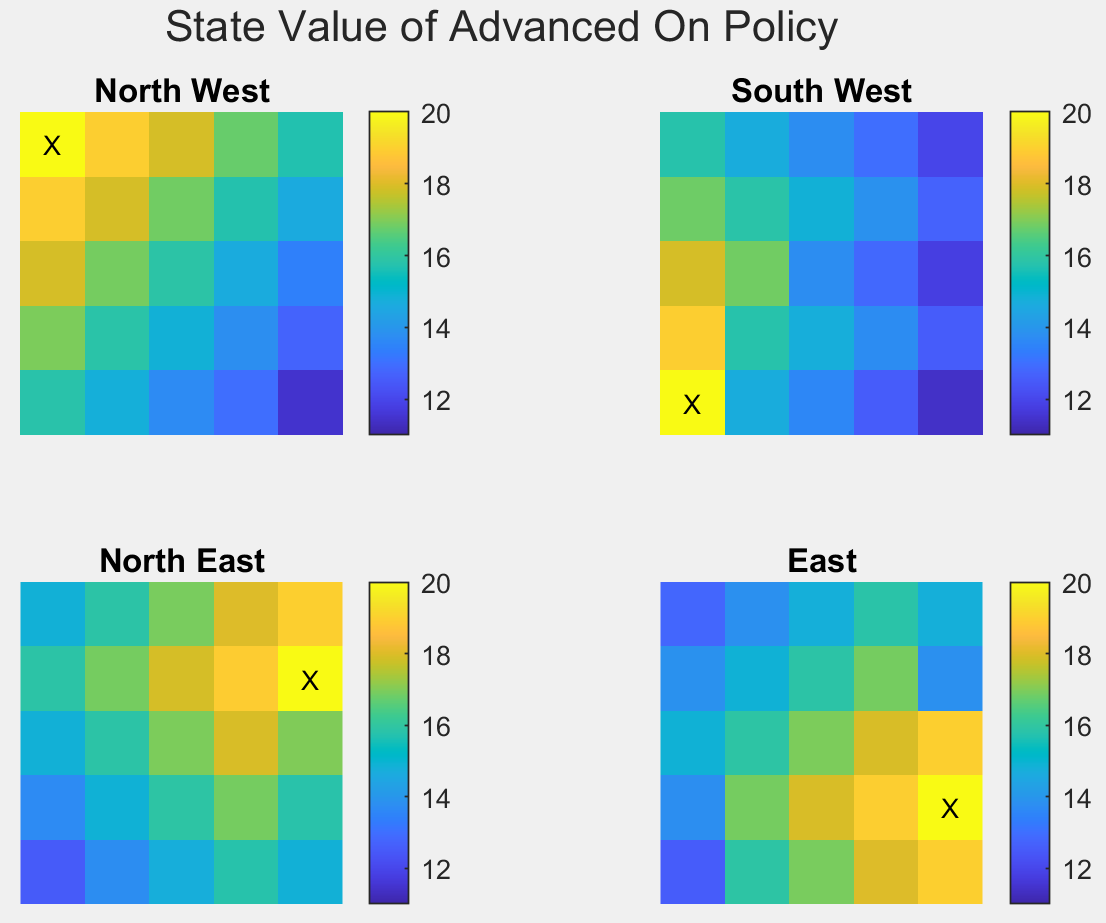
\includegraphics[width=0.9\linewidth]{pics/Aonp_state_val.PNG}
    \caption{\centering Color map of advanced on-policy estimated state value for different package positions}
    \label{fig:Aonp_sv}
\end{figure}

igure \ref{fig:comp} presents the average return per episode for three Monte Carlo control strategies: standard on-policy, off-policy, and advanced on-policy. Each curve represents the agent’s learning performance over 100,000 episodes, providing insight into how quickly and effectively each method converges toward optimal behavior.

The first subplot shows the performance of the standard on-policy method using a constant $\epsilon$-greedy strategy. The return starts low—around –30 to –40—due to frequent illegal actions and inefficient paths in early exploration. Over time, the average return improves and eventually stabilizes, although it remains noisy and does not consistently reach the optimal return level. This indicates that the agent struggles to fully converge due to suboptimal updates caused by early exploratory actions.

The second subplot illustrates the off-policy Monte Carlo method with importance sampling. This approach quickly achieves near-optimal performance, with the average return rising sharply and stabilizing early in the learning process. The results confirm that the off-policy method is more stable and effective in learning optimal actions, even when sampling trajectories from a separate behavior policy.

The third subplot shows the results for the advanced on-policy method, in which the learning is broken into several smaller phases with decreasing $\epsilon$ values in each phase. This structured approach allows the agent to quickly correct early mistakes and refine its policy with greater precision in later phases. As a result, the average return rises sharply and stabilizes at an optimal level, closely matching the off-policy performance. This demonstrates that the advanced on-policy approach can significantly improve convergence and learning efficiency without relying on importance sampling.


\begin{figure}
    \centering
    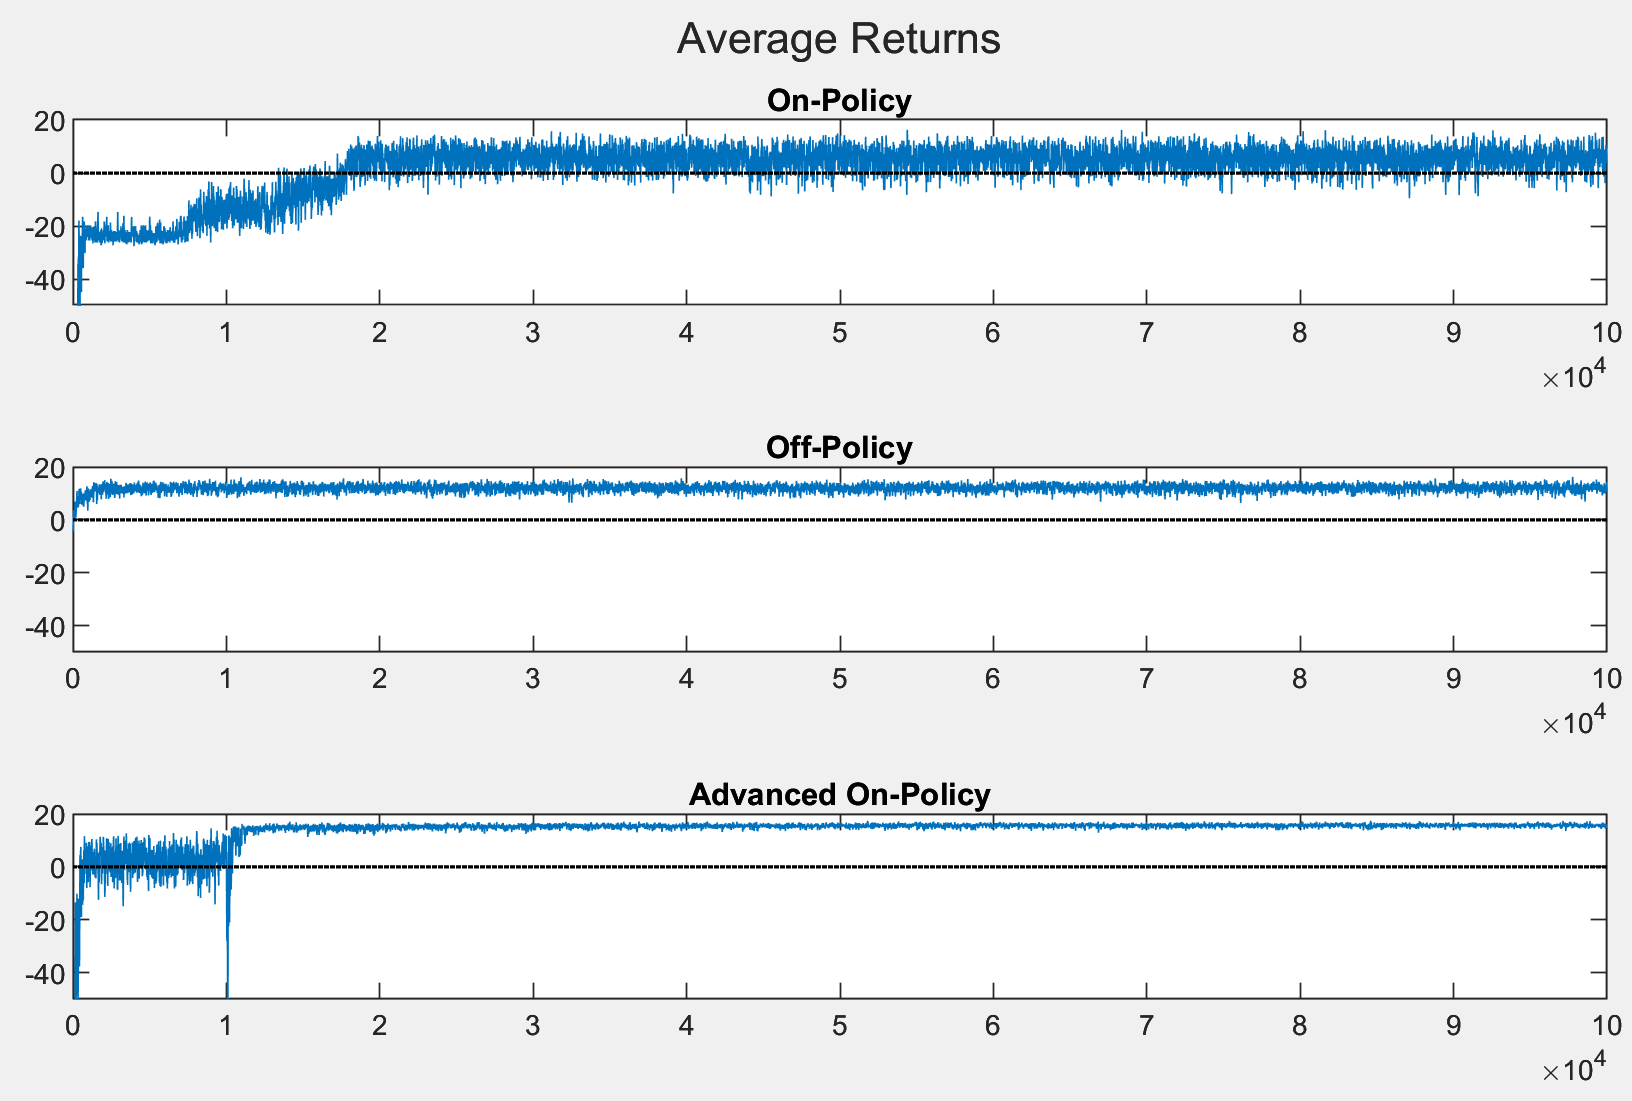
\includegraphics[width=0.9\linewidth]{pics/comp.PNG}
    \caption{\centering Average rewards of different control method over all episodes}
    \label{fig:comp}
\end{figure}


%%%%%%%%%%%%%%%%%%%%%%%%%%%%%%%%%%%%%%%%%%%%%%%%%%%%%%%%%%%%%%%%%%%%%%%%%%%%%%%%%%
%                  Conclusion
%%%%%%%%%%%%%%%%%%%%%%%%%%%%%%%%%%%%%%%%%%%%%%%%%%%%%%%%%%%%%%%%%%%%%%%%%%%%%%%%%%
\section{Conclusion}
The results illustrate the comparative learning performance of three Monte Carlo control strategies applied to a gridworld delivery task. The standard on-policy method shows a gradual improvement in average return over the first 20,000 episodes, eventually stabilizing around a suboptimal level with noticeable variance. This reflects the method’s sensitivity to early exploratory actions, which may bias the value estimates and slow convergence.\par

In contrast, the off-policy approach demonstrates much faster and more stable convergence. Average returns reach near-optimal values within the first few thousand episodes and remain consistently high thereafter, confirming the robustness of off-policy learning with importance sampling in efficiently estimating optimal policies.\par

The most striking result is observed with the advanced on-policy method, which breaks the training process into multiple smaller phases with decreasing $\epsilon$. This staged training strategy enables the agent to rapidly recover from early mistakes and converge to near-optimal behavior almost as quickly as the off-policy method. The sharp rise in returns around the 10,000th episode and their stability over time indicate that this approach effectively addresses the shortcomings of standard on-policy control. Thus, the advanced on-policy variant combines the simplicity of on-policy learning with performance close to off-policy methods, making it a practical and effective alternative.\par


\vfill

\end{document}


